\chapter{Experimental setup}

\intro{The measurements within this thesis are based on \glsreset{pp}\gls{pp} collision data recorded with the CMS detector in 2012, 2015, and 2016 at center-of-mass energies of 8 and 13~\TeV. The experimental setup is described in this chapter. First, the \gls{lhc}, its preacceleator chain and other experiments at the \gls{lhc} are briefly introduced. Then, the CMS detector and its components are detailed. A review of the operations summarizes the chapter.}

%##############################################
\section{Large Hadron Collider}
%##############################################

The \glsreset{lhc}\gls{lhc} is a 26.7~km long accelerator and storage ring for \glsreset{proton}\glspl{proton} and \glsreset{ion}\glspl{ion} at the \glsreset{cern}\gls{cern} located in the vicinity of Geneva, Switzerland. It was constructed between 1998\range2008 in the existing tunnel of the former \glsreset{lep}\gls{lep} which lies 45\range170~m below the surface. The \gls{lhc} ring features two beam pipes which can be separately filled with up to 2'808 countercycling bunches of protons with a bunch-to-bunch spacing of 25~ns per pipe. The beams can be focused for crossing each other at four \glspl{ip} where however only two of them are meant for a high luminosity collisions. The design allows to accelerate protons with a momentum of 450~\GeV at injection to up to 7~\TeV yielding a center-of-mass energy of 14~\TeV in collisions.

To bend the beams 1'232 dipol cryostats are deployed hosting both beam pipes and two dipol magnets within a cold mass in a twin-bore design. The cold mass itself is placed in a vacuum vessel for thermal insulation. The magnet coils consist of \gls{nbti} alloy fibers which are cooled down to 1.9~K using superfluid helium. At this temperature, the magnets are superconducting. This allows to produce the required magnetic field strength to sustain a closed beam orbit ranging from 0.54~T at injection energy to up to 8.33~T for the maximum beam energy. At maximum field a current of 11850~A is required. Such high magnetic fields cannot be achieved with normal conductors due to magnetic saturation. 

Additional about 3'800 single aperture and 1'000 twin aperture magnets are installed. Quadrupole magnets keep the beam particles focused around the nominal orbit. Further, non-linear corrections to the orbit are applied using sextu-, octu-, and decapoles. Special quadrupole triplets at each side of the four \glspl{ip} focus the beams for collision. The envelop of the particle trajectories with respect to the nominal beam orbit is described by the beta function which can be approximated around the \glspl{ip} as 

\begin{equation}
\beta(x)\approx\beta^\star+\frac{x^2}{\beta^\star}.
\end{equation}

In design, the beams can be squeezed to $\beta^\star=0.55~\mathrm{m}$ at the two high luminosity \glspl{ip}. The transverse beam size is given as $d^{\star}=\sqrt{\epsilon_\mathrm{n}\cdot\beta^\star/\gamma}\approx17\upmu\mathrm{m}$ for $\gamma=E_\mathrm{p}/m_\mathrm{p}=7000$ where $\epsilon_\mathrm{n}$ denotes the normalized beam emittance. It is a measure of the phase space area occupied by the particles within the beam which is constant following Liouville's theorem. The emittance cannot be larger than $\epsilon_\mathrm{n}>3.75~\upmu\mathrm{m}\cdot\mathrm{rad}$ in order to not loose significant amounts of the beam in the \gls{lhc} arcs where $\beta(x)$ is the largest.

For acceleration and longitudinal focusing, a system of eight superconducting cavity per beam with a resonance frequency of $400.8~\mathrm{MHz}$ are installed. This matches the 35640~harmonic mode of the beam revolution frequency of $f_\mathrm{rev}=11'245~\mathrm{Hz}$. The cavity system yields an energy gain per turn of 485~keV which results in an acceleration time of about 20~min from injection to the maximum beam energy.

The expected luminosity at the \glspl{ip} can be calculated from the introduced machine and beam parameters as

\begin{equation}
L=\frac{N_\mathrm{p}^{2}n_\mathrm{b}f_\mathrm{rev}}{4\pi\,d^{\star 2}}\cdot F,\qquad F=1\Bigg/\sqrt{1+\Big(\frac{\theta\cdot d_{z}}{2\,d^\star}\Big)^2}
\end{equation}

where $N_\mathrm{p}$ denotes the number of protons per bunch and $n_\mathrm{b}$ the number of colliding bunches. Typical bunch intensities are $N_\mathrm{p}=???$. \todo{what?} The factor $F$ accounts for a reduction in luminosity due to the slightly tilted beams by the crossing angle $\theta$.

In 2016, the design luminosity of $10^{34}~\mathrm{cm}^{-2}\mathrm{s}^{-1}$ was surpassed through various new developments~\cite{Team:2229040}. In detail these were a decrease of the transverse emittance, a smaller longitudinal bunch size, a better focusing at the \glspl{ip} down to $\beta^\star=0.4~\mathrm{cm}$, and a smaller crossing angle compared to the design values. This resulted in a peak luminosity of $1.5\cdot 10^{34}~\mathrm{cm}^{-2}\mathrm{s}^{-1}$. An overview of the peak luminosity in recorded \gls{pp} collisions by the CMS experiment from 2010--2016 is shown in Fig.~\ref{fig:experiment-peaklumi}. More information on the \gls{lhc} and its design parameters can be found in Ref.~\cite{Evans:2008zzb}.

\myfigure{\label{fig:experiment-peaklumi}Peak luminosity in proton-proton collision data per day recorded by the CMS experiment. The figure is taken from the public luminosity result web page of CMS~\cite{lumipublic}.}{
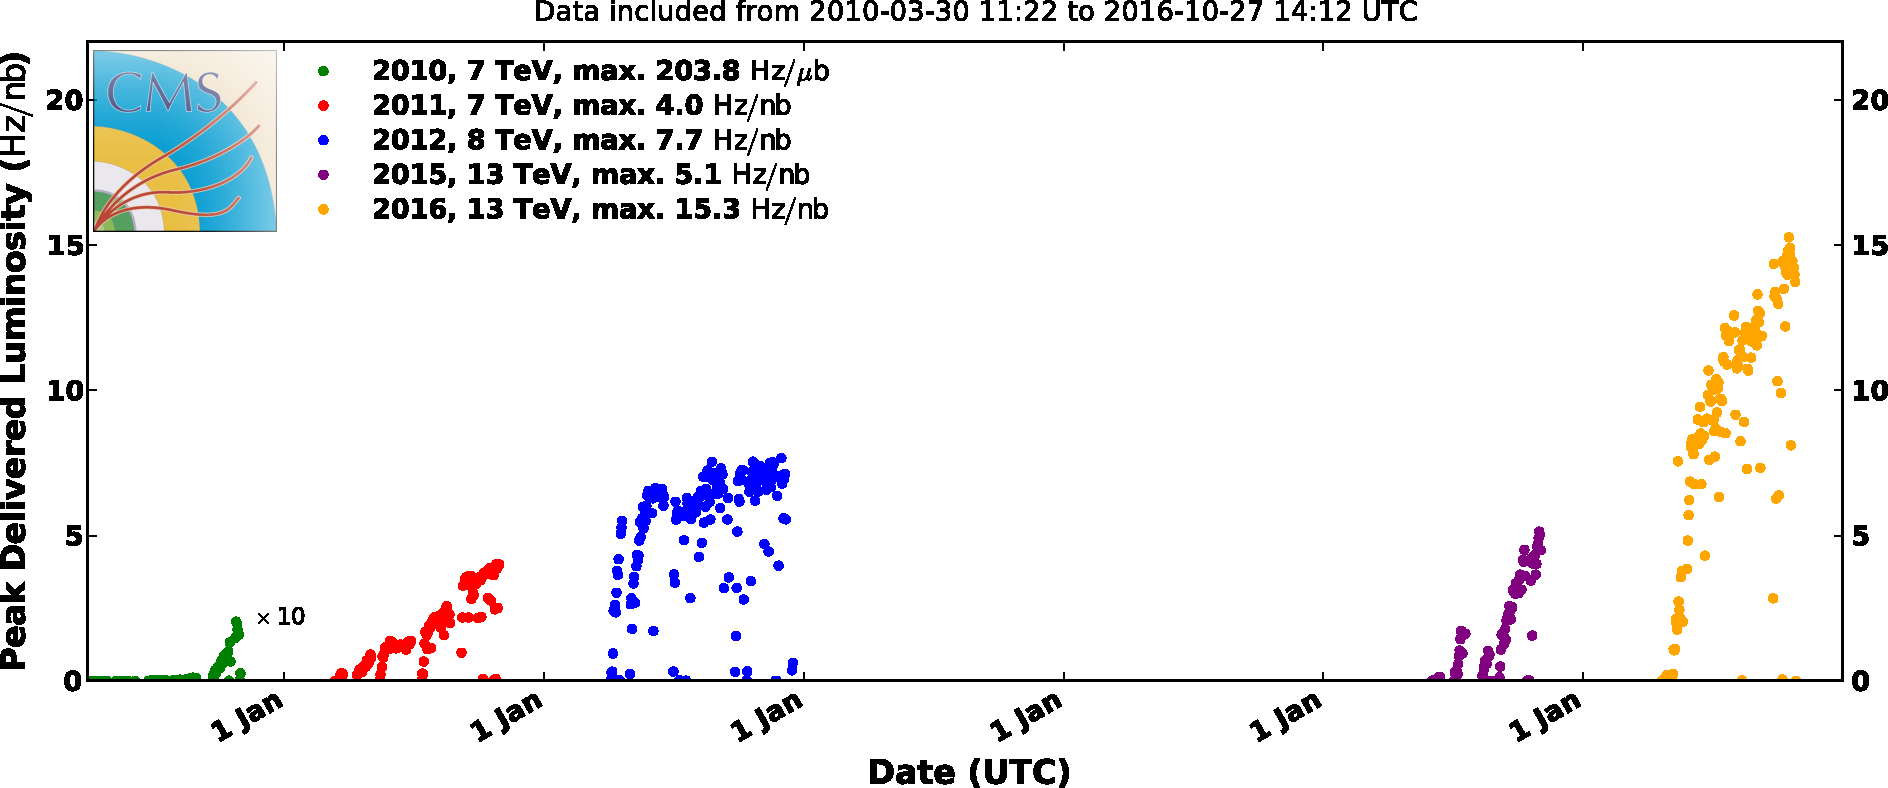
\includegraphics[width=0.95\textwidth]{figures/experiment/peak_lumi_pp.pdf}
}

During a bunch crossing multiple proton-proton interactions can occur which are referred to as \gls{pu}. Their number on average is proportional to the luminosity and the total inelastic \gls{pp} cross section. In 2012, an average number of 21 pileup interactions has been observed in 8~\TeV \gls{pp} collisions. This increased in 2016 due to the higher luminosity and cross section at 13~\TeV to ??? interaction per bunch crossing. \todo{no pu number found}

\todo{add short overview of operation and energies and delivered lumis}

%##############################################
\subsection{Accelerator complex}
%##############################################

An overview of the accelerator complex at \gls{cern} is given in Fig.~\ref{fig:experiment-accelerator-complex} which includes the systems for filling the \gls{lhc} with bunches of protons or lead ions.

\myfigure{\label{fig:experiment-accelerator-complex}The accelerator complex at \gls{cern}. The figure is taken from Ref.~\cite{Mobs:2225847}.}{
%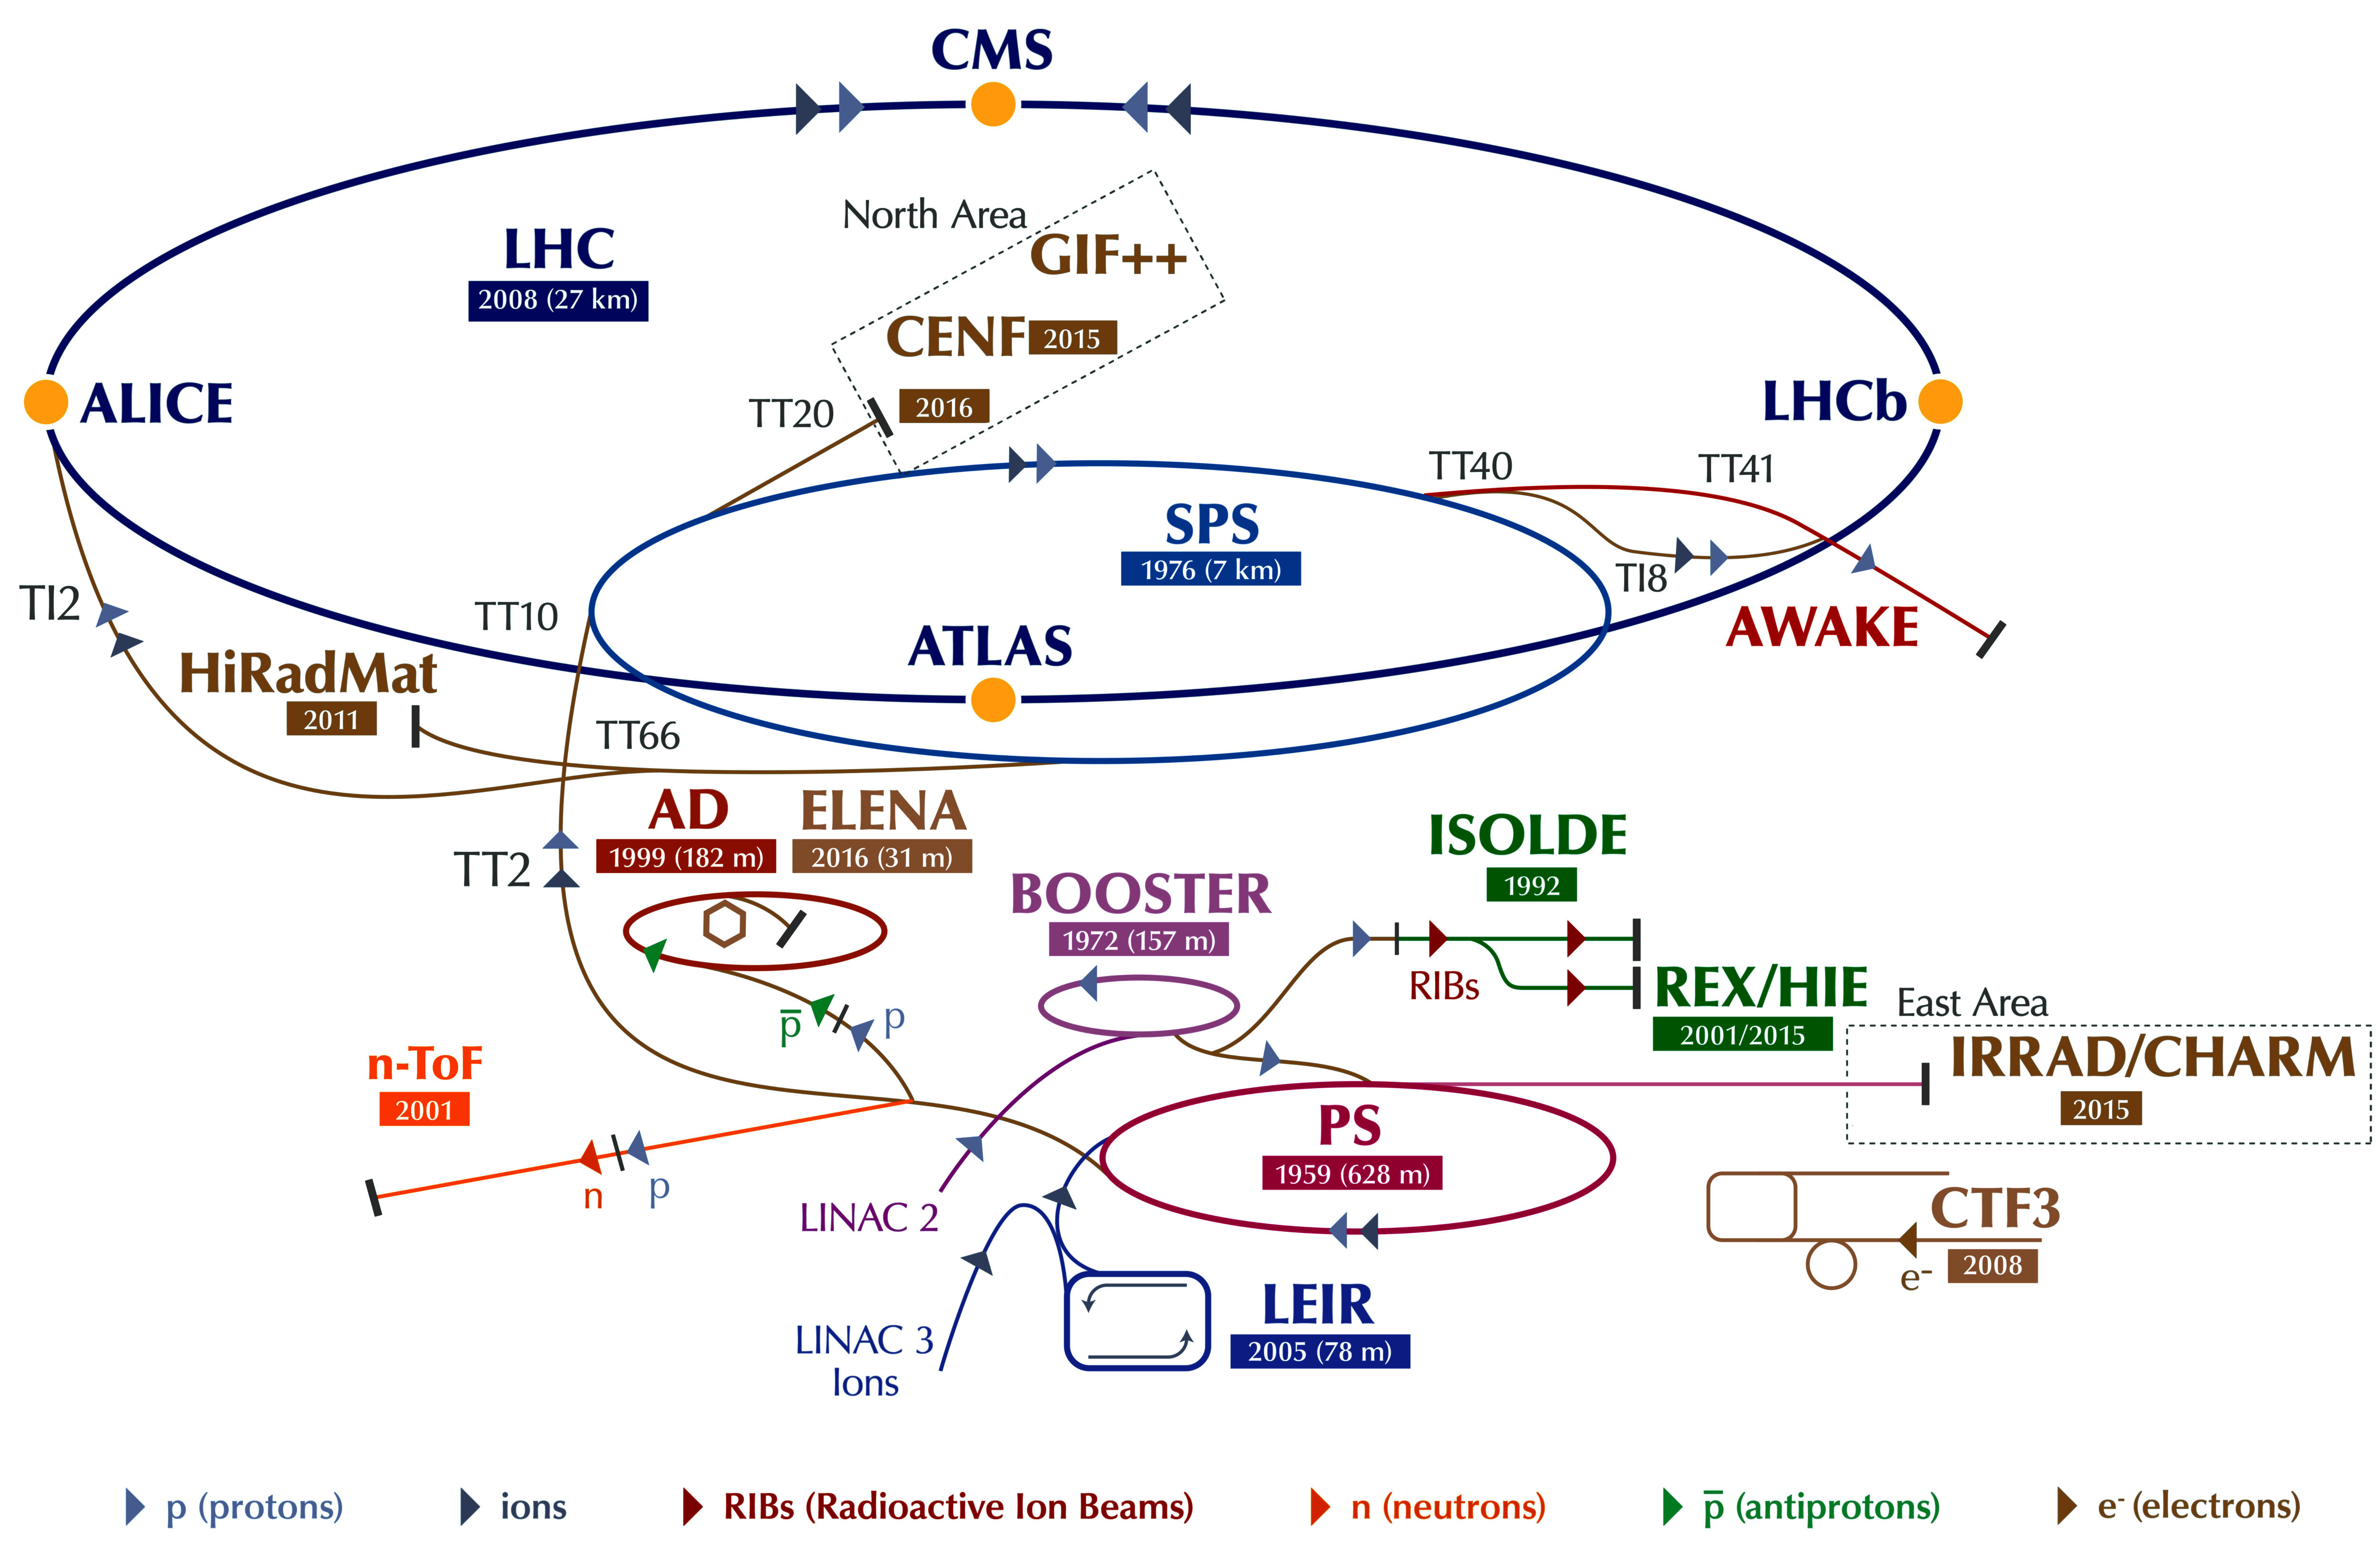
\includegraphics[width=0.99\textwidth]{figures/experiment/CERN_accelerator_complex.jpg}
}

The production sequence of proton bunches for the \gls{lhc} is as follows. In the linear accelerator ``Linac~2'', hydrogen atoms are stripped of their electron through an electric field. The remaining protons are accelerated to a momentum of 50~\MeV and injected into the \glsreset{psb}\gls{psb}. It consists of four vertically separated beam pipes which allow multi-turn injections to increase the bunch intensity which however also increases the transverse emittance~\cite{doi:10.1142/S0217751X13300196}. After accelerating the protons to 1.4~\GeV, the beams are injected into the \glsreset{ps}\gls{ps}. Here the required bunch spacing of 25~ns is formed. Until recently the standard procedure was to use only six bunches from two \gls{psb} cycles and split them first by three, accelerate them to 25~\GeV, and then split each again by two twice to produce in total 72~bunches with the required spacing~\cite{Benedikt:2001ar}. A new scheme called \gls{bcms} was introduced in 2016. It utilizes all eight bunches from two \gls{psb} cycles which are first narrowed and then combined to four followed by the same splitting and acceleration procedure as before which results in 48~bunches with higher intensity and lower transverse emittance~\cite{bcms}. Finally, the protons are injected and accelerated in the \glsreset{sps}\gls{sps} up to the \gls{lhc} injection energy of 450~GeV.

\todo{gap? beam life and filling time?}

%##############################################
\subsection{Overview of experiments}
%##############################################

Various particle detectors are installed at the \gls{lhc} to record the outcome of proton-proton, proton-lead, and lead-lead collisions. Four major detectors are directly located at the \glspl{ip}. 

Two general purpose detectors are located at the two high luminosity \glspl{ip}. These are the \gls{atlas}~\cite{Aad:2008zzm} and \gls{cms}~\cite{Chatrchyan:2008aa} experiments which have both a wide physics program ranging from precision measurements of the \gls{sm} to the search for various kinds of new physics like extra dimensions, dark matter particles or \gls{susy}. Despite similar goals the technical realization of the two experiments is different. The \gls{atlas} detector is of cylindrical shape around the beam pipe with a length of 44~m and a diameter of 25~m. It consists of an inner detector, a liquid argon electromagnetic calorimeter, a hadronic calorimeter, and a muon spectrometer with full $2\uppi$ coverage in the azimuthal angle. %The inner detector is placed within a solenoid producing a magnetic field of 2~T for tracking of charged particles. A toroidal magnetic field with an average strength of 0.5~T allows to determine the momenta of muons in the outer spectrometer. 
Detailed information on the \gls{cms} detector are given in Sec.~\ref{sec:experiment-cms}.

The two other major detectors are the \gls{alice}~\cite{Aamodt:2008zz} and \gls{lhcb}~\cite{Alves:2008zz} experiments which are more specialized. 

In addition to the four major experiments, three 

%##############################################
\section{CMS experiment}
%##############################################
\label{sec:experiment-cms}

\myfigure{The figure is taken from Ref.~\cite{Bayatian:2006zz}.}{
%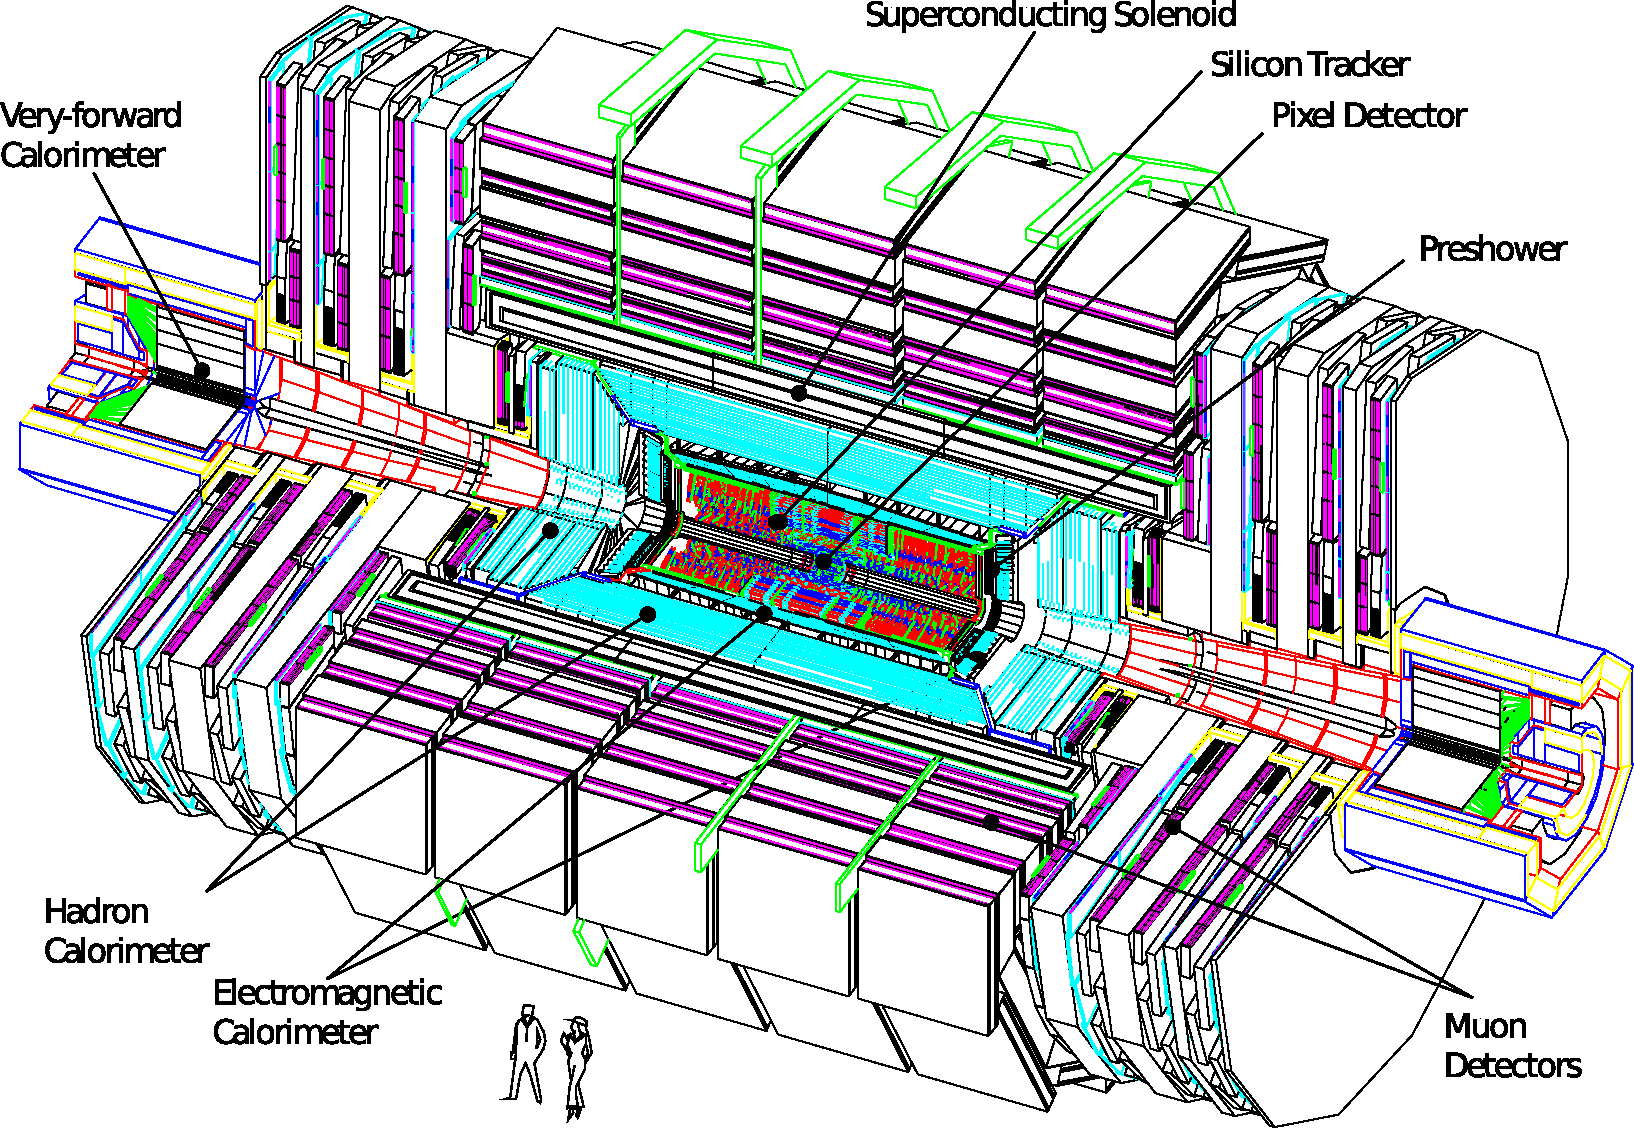
\includegraphics[width=0.99\textwidth]{figures/experiment/CMS_overview.pdf}
}

%##############################################
\subsection{Magnet}
%##############################################

\cite{Acquistapace:1997fm}

%##############################################
\subsection{Tracker}
%##############################################



\cite{Chatrchyan:2014fea}

%##############################################
\subsection{Electromagnetic calorimeter}
%##############################################

%##############################################
\subsection{Hadronic calorimeter}
%##############################################

%##############################################
\subsection{Muon systems}
%##############################################
DT/RPC/CSC

%##############################################
\subsection{Data acquisition}
%##############################################
Trigger/DAQ

%##############################################
\subsection{Operations}
%##############################################
DCS/DSS
